\section{Properties of Square Lattice Graphs}
\begin{lemma}
Every vertex $v\in V$ of a square lattice graph $G=(V,E)$ representing a closed boundary, must have a degree $d(v)\geq 2$.\label{DegreeLemma}
\end{lemma}
\subsubsection*{Proof of Lemma~\ref{DegreeLemma}}
If a vertex $v\in V$ has degree $d(v)=0$, and the number of vertices $\in V>1$, then that vertex cannot connect to any other vertices in the square lattice graph, and can thus not form part of the closed boundary. If a vertex $v_0\in V$ has degree $d(v_0)=1$, then any path $p$ where $v\in p$, will not be a Hamiltonian cycle, as the edge $e\in E$ where $v_0\in e$, can only be crossed once, as the adjacent vertex $v_1\in e$, can only be crossed once on path $p$.\autocite{myself}
\begin{lemma}
For all vertices $v\in V$ of a square lattice graph $G=(V,E)$, where $d(v)=2$, each of its edges must be included in a Hamiltonian cycle of $G$.\label{TwoEdgesLemma}
\end{lemma}
\subsection*{Proof of Lemma~\ref{TwoEdgesLemma}}
In a Hamiltonian cycle of graph $G$, one of the edges of $v$ must be required for it to be included in the cycle. A walk that crosses the same edge twice must include the same vertex twice, since for each edge in a walk, both connecting vertices are included in the walk, which cannot apply for a Hamiltonian cycle. As the Hamiltonian cycle is a cycle, $v$ cannot be a dead end. Thus, both edges of $v$ must be included within any resulting Hamiltonian cycle.
\begin{lemma}
In a square lattice graph of a closed boundary wall configuration, in relation to the vertices' grid coordinates, out of the northernmost vertices, the westmost vertex will always be a corner connecting two vertices to its east and its south, respectively.\label{NorthwestCornerLemma}
\end{lemma}
\subsubsection*{Proof of Lemma~\ref{NorthwestCornerLemma}}
In such a lattice graph, we pick the westmost vertex amongst the northernmost vertices. If there is a vertex connected to it, to its north, then our chosen vertex was not the northernmost vertex which is a contradiction. If there is a vertex connected to its west, then it is not the westmost vertex and is again a contradiction.\autocite{myself}
\begin{conjecture}
A square lattice graph of a closed boundary wall configuration will always have at least 4 corner vertices, each connecting to two vertices, and each pointing into different cardinal directions.\label{FourCornerLemma}
\end{conjecture}
\subsubsection*{Justification of Conjecture~\ref{FourCornerLemma}}
Following from theorem~\ref{NorthwestCornerLemma}, in a square lattice defining a boundary there is at least one corner corner vertex $v_{se}$ with an edge to its east and one to its south. Since by definition there are no vertices $v\in V$ that are to the north of $v_{se}$, there must be a vertex to its east, directly connected to it by a straight walk, that is a corner vertex $v_{sw}$ with an edge to its south and to its west. 
\\Firstly, we define each cardinal direction to consecutive integers. North$\leftarrow$0, East$\leftarrow$1, South$\leftarrow$2, and West$\leftarrow$3. We also define the normal of a direction as $Normal(d)= d+3 \pmod{4}$. This normal will always point opposite towards the direction needed to complete a full cycle, based on the current walking direction. We get the opposite of a direction through $Opposite(d)=d+2\pmod{4}$.
\\Starting from $v_{se}$ we can walk east until there is a vertex that only connects southwards. The walk progresses southwards. If a vertex that connects eastward, or of $Normal(South)$ is encountered, we follow that walk until there is a walk towards $Normal(Normal(South))$, and so and so forth evaluated recursively, until we encounter a corner wall that points towards $Opposite(Normal(currentDirection))$, where $currentDirection$ is the direction walked from the second last vertex of the walk. We again assume a new direction of walking, and always recursively iterate through any vertices connecting to $Normal(currentDirection)$, until only its opposite can be continued on.
\\The recursive iteration, always taking the above-defined normal function, will take the form of an inward spiral. The spiral is limited in extent, as it cannot exceed the northernmost vertices, by definition, and the lengths of the spiral must shorten after every turn. This cannot continue indefinitely, and must thus ''unwind'' again. Eventually iterating through all vertices. At some point the $Opposite(Normal(currentDirection))$ must be encountered for all $currentDirection$. Thus there must be at least 4 corners which point in this direction, for a Hamiltonian cycle to exist.\autocite{myself}
\\This conjecture is well illustrated in the Figures ~\ref{SpiralLevel} and ~\ref{SpiralLevelOutcome}.
\begin{figure}[H]
	\centering
	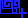
\includegraphics[width=0.6\linewidth]{Image-9.png}
	\caption {Spiral level blueprint\autocite{myself}}\label{SpiralLevel}
\end{figure}
\begin{figure}[H]
	\centering
	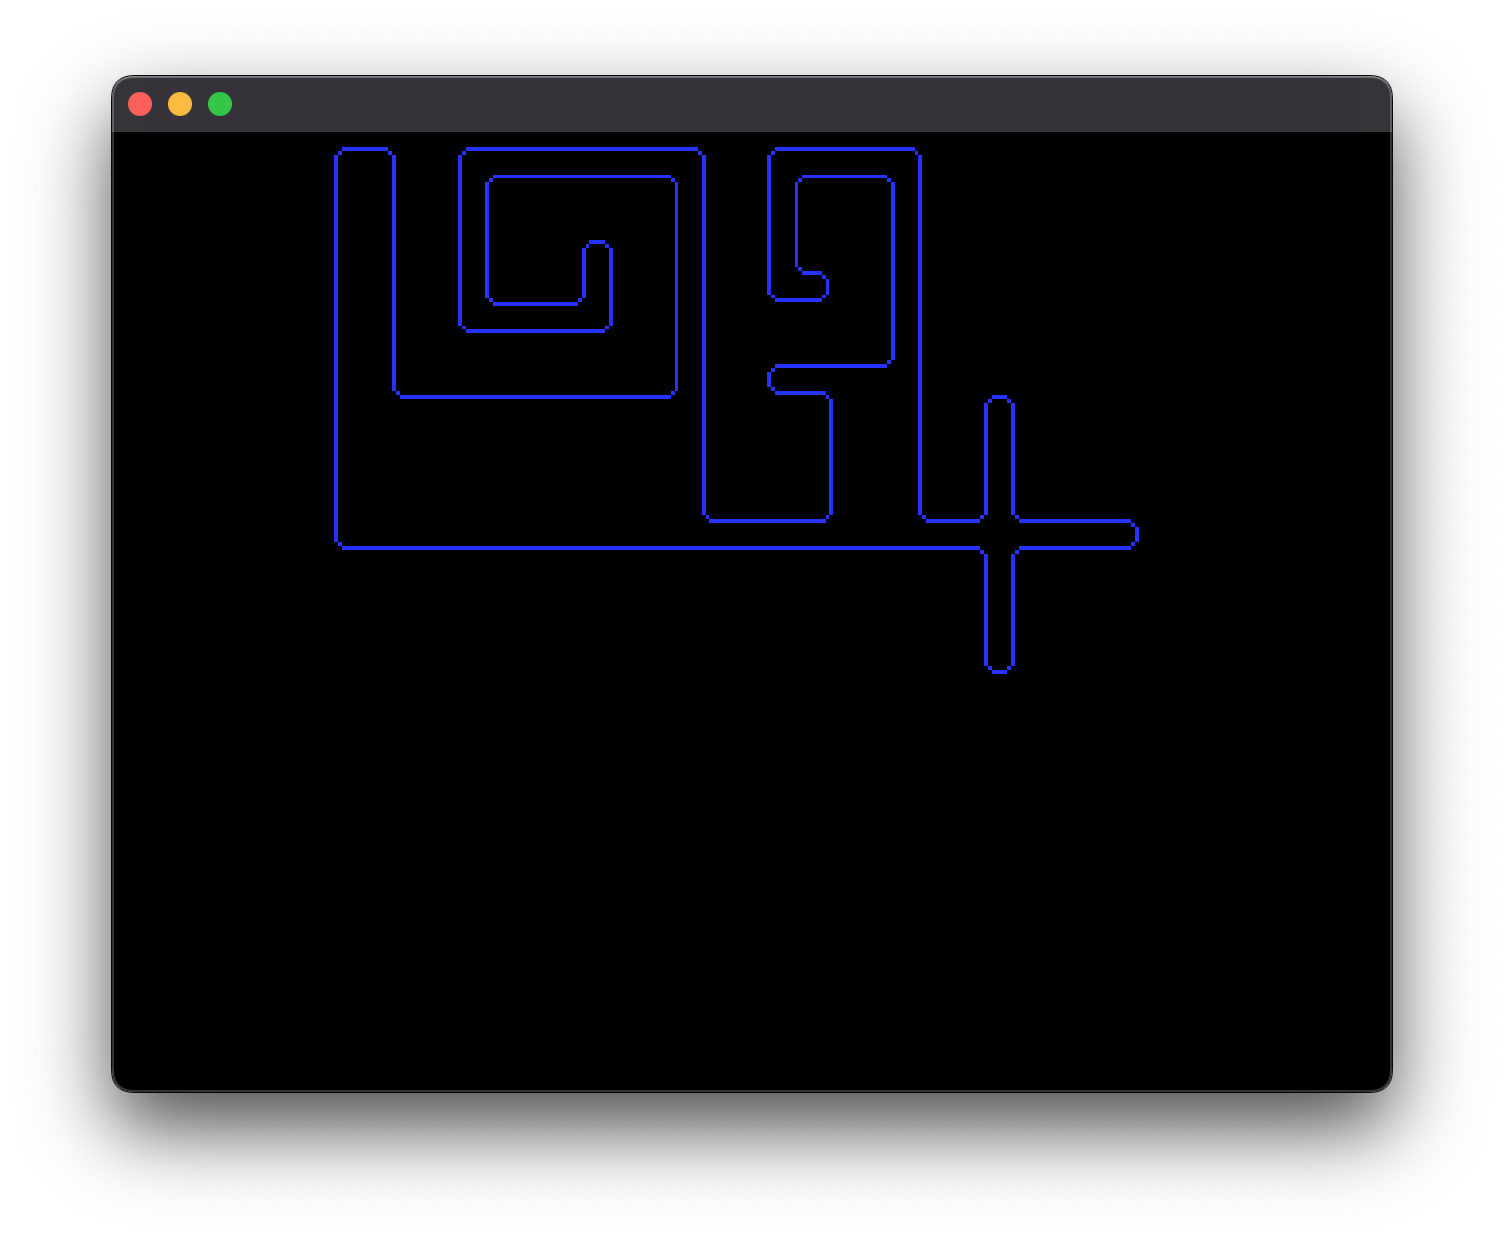
\includegraphics[width=0.8\linewidth]{Image-10.png}
	\caption {Spiral level output\autocite{myself}}\label{SpiralLevelOutcome}
\end{figure}
